\section{Introduction}
Recently, there has been a surge of interest with regards to reinforcement learning in the machine learning community which has demonstrated significant progress on performing several tasks successfully, most notably on games such as for Atari~\cite{mnih2015human} and the board game Go~\cite{silver2016mastering}. The key to their success was combining deep convolutional neural networks~\cite{krizhevsky2012imagenet} with model-based reinforcement learning~\cite{sutton1998reinforcement}. In my paper, I experiment with model-based reinforcement learning by adding a hierarchical component and demonstrate their benefits.

\subsection{Reinforcement Learning}
Reinforcement learning (RL) is a machine learning technique where an agent learns through reward and punishment. RL is inspired by how animals learn. Animals learn to associate actions with positive and negative feedback. In animals, the likelihood of an animal executing an action associated with positive feedback increases and decreases with negative feedback. Just like in humans, RL agents are more likely to perform actions that result in the most positive feedback (known as reward) over time. 

Over the years, researchers have formalized RL with equations designed to capture the essence of animal reinforcement learning. At its core, an RL model is typically a markov decision process where the model has a set of states \textbf{s}, a set of actions \textbf{a}, a transition function \textit{T(s,a)}, a reward function \textit{R(s,a)}, and a way for the agent to observe the environment.

There are many implementations of RL which can broadly be divided into two categories, model-based and model-free, then within these categories there are futher sub-divisions such as on-policy or off-policy, fully observable or partially observable etc. The choice of which depends on the goals of the problem and how knowledgeable the agent is of its environment.

\subsubsection{Model-based}
Model-based RL is where the agent has complete knowledge of the transition function and reward function. Essentially, the agent has a map of the world for which it can learn the best actions. RL methods such as policy iteration take advantage of this fact by perform dynamic programming which is guaranteed to converge. The advantage of this approach is that there is a guaranteed solution, the downside is that not every problem comes with knowledge of the transition and reward functions.

\subsubsection{Model-free}
Model-free RL models lack the knowledge of the environment's transition and reward functions. Therefore, model-free models must learn the best state-action pairs by sampling the environment's states. The sampling is performed by sometimes stochastic selection of actions.
 
\paragraph{Temporal Difference Learning}
Temporal difference (TD) learning is a popular model-free algorithm. Each state and action pair has a value $V$ associated with it. The agent will take the action with the maximum $V$ value. To learn, when an agent takes an action $a$, the agent calculates the difference between the current estimate of the value function \textbf{V($s$)} and the reward from $a$ plus the estimated value at the next state \textbf{V($s_{next}$)}. This difference (delta) is either positive or negative signifying that the agent's value of the current state should be higher or lower respectively. The values of each state are then adjusted accordingly. The full equations are presented below: 

\begin{equation}\delta = r_{t+1} + \gamma V(s_{t+1}) - V(s_{t})\end{equation}

\begin{equation}V(s_t) \Longleftarrow V(s_t) + \alpha\delta\end{equation}

where alpha is the learning rate and gamma is the discount factor.

\subsubsection{Actor Critic Model}
The specific model architecture I use in my paper is the actor-critic model. This particular model separates the decision making process from the value function. Each state has a set of weights for each action and a value. When an action is made and the delta is calculated, both the action weights \textbf{W} and the current state's value $V$ are updated. Figure \ref{fig:actor-critic} demonstrates an example of the Actor Critic Model.

% \begin{figure}[h]
% \centering
% 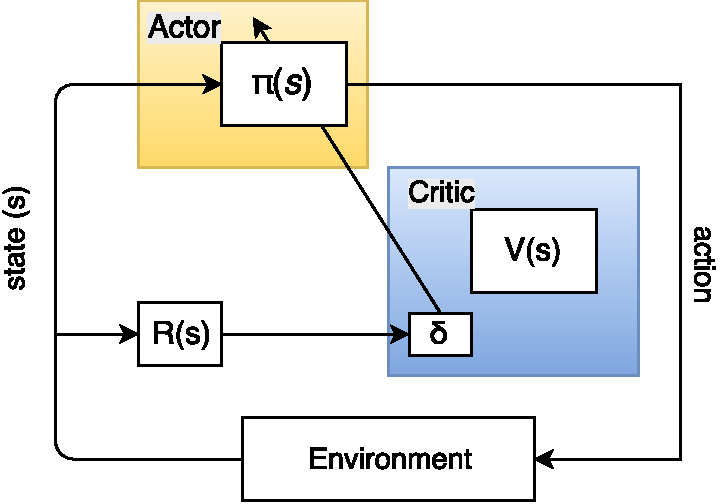
\includegraphics[scale=0.4]{actor-critic.pdf}
% \caption{The actor critic model. $\pi$ represents the policy of the actor. V(s) represents the value function. $\delta$ represents the prediction error. R(s) represents the reward function.}
% \label{fig:actor-critic}
% \end{figure}

% \begin{figure}[h]
% \centering
% 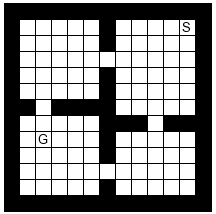
\includegraphics[scale=0.4]{environment.png}
% \caption{The environment composed of four rooms. The goal state is marked with a G. The start state is marked with an S.}
% \label{fig:environment}
% \end{figure}

\begin{figure*}[h]
    \centering
    \begin{subfigure}[h]{0.49\textwidth}
        \centering
        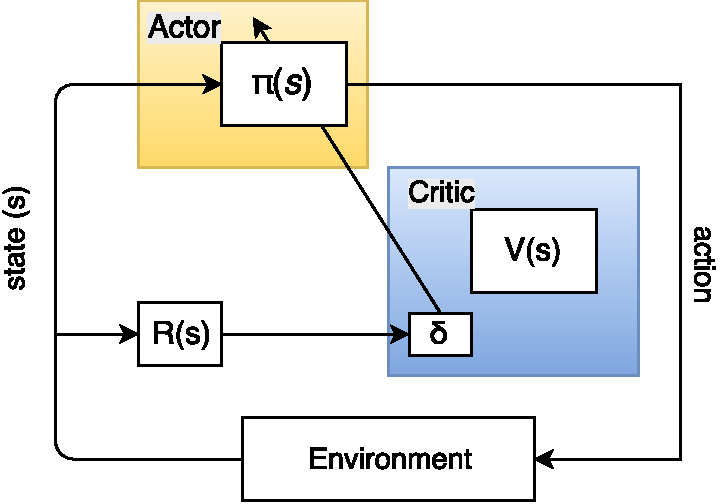
\includegraphics[scale=0.49]{actor-critic.pdf}
        \caption{The actor critic model. $\pi$ represents the policy of the actor. V(s) represents the value function. $\delta$ represents the prediction error. R(s) represents the reward function.}
		\label{fig:actor-critic}
    \end{subfigure}%
    ~ 
    \begin{subfigure}[h]{0.49\textwidth}
        \centering
        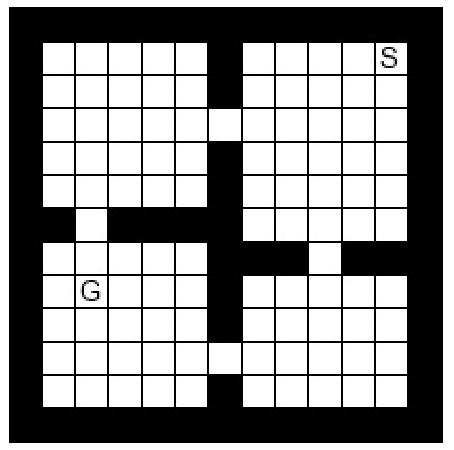
\includegraphics[scale=0.49]{environment2.pdf}
        \caption{The environment composed of four rooms. The goal state is marked with a G. The start state is marked with an S.}
		\label{fig:environment}
    \end{subfigure}
\end{figure*}

\subsection{The Scaling Problem}
The problem with RL is that as the number of actions and states increases, the training time also increases at an accelerating rate \cite{botvinick2009hierarchically}. For simple problems, RL can perform well but for more complex problems involving millions of states and hundreds of actions, the problem can quickly become intractable. There have been different attempts to address this problem. Some researchers have abstracted the states into similar groupings~\cite{li2006towards}, or others have proposed temporally abstract actions~\cite{sutton1999between}. These temporally abstract actions are essentially a separate policy that is followed until a sub-goal state is reached at which point the original higher-level policy resumes control. Temporally abstract actions form the basis of Hierarchical Reinforcement Learning (HRL).

\subsection{Hierarchical Reinforcement Learning}
HRL has several implementations, the implementation I use is taken from Botvinick's previous work~\cite{botvinick2009hierarchically}. It is an actor-critic model. In his implementation, temporally abstract actions are known as options. Actions can thus be either primitive actions or options following their own policy. When an option reaches one of its sub-goals it returns control back to the original root policy. 

To learn an option's policy, the agent receives a pseudo-reward for reaching a sub-goal. Pseudo rewards are separate from external environmental rewards. Peudo-rewards allow the agent to learn the best way possible to reach their options terminating state i.e. sub-goal, regardless of the amount of external reward.

When an option terminates at state $s$, the control of the agent is returned to the higher order root option. The initial root option's policy is updated with the cumulative external reward for selecting option $o$ at the initial state $s_{init}$. $s_{init}$ represents the state at which the option $o$ was first selected. Figure~\ref{fig:state-transitions} demontrates an example of an agent moving using options.

\begin{figure}[h]
\centering
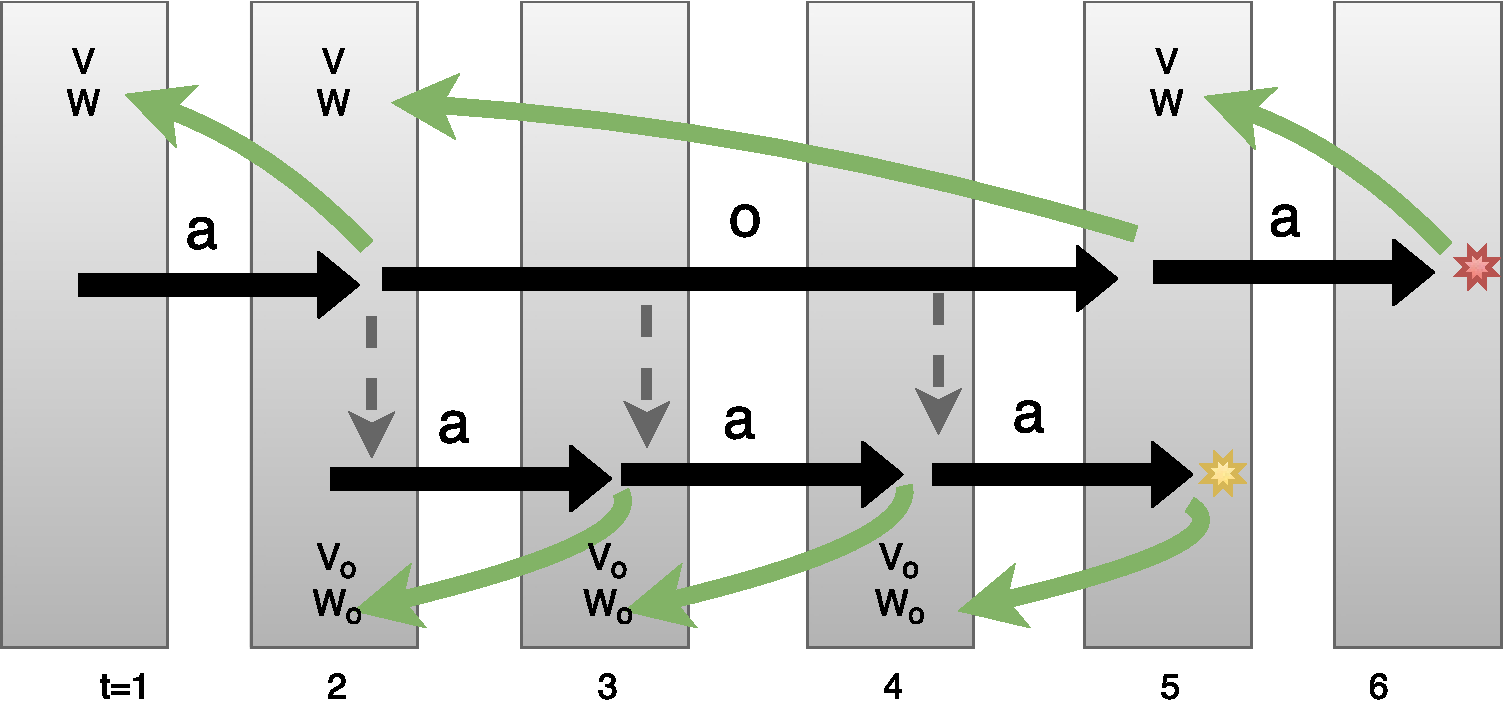
\includegraphics[scale=0.3]{state-transitions.pdf}
\caption{State transitions for a hierarchical RL model using options. When an action is made at the root option level, the value and action weights are updated for the previous state and receive external reward (red star). When an option is selected, the options policy is followed and the option's value and action weights are updated using pseudo reward (the yellow star). Also, when an option finishes, the value and action weights at the root option level are updated to account for how well the agent performed selecting the option.}
\label{fig:state-transitions}
\end{figure}

The benefit of HRL is two-fold. The first benefit is that HRL reduces the size of the search space. Many successive branches of the search tree are abstracted to a single branch by using options. The result of choosing an option skips primitive actions in the tree. The second benefit is that HRL has fewer parameters to tune resulting in a less complex model. A less complex model is easier to train and understand. For example, performing two sucessive options (each composed of four actions) results in only two parameters being tuned at the root level versus peforming eight successive primitive actions which each require tuning.

\section{Related Work}
Sutton introduced HRL and demonstrated a working implementation in his book~\cite{sutton1999between}. Botvinick applied HRL and discussed the neural basis of humans performing HRL~\cite{botvinick2009hierarchically}. However, he did not perform model-based learning. Diuk et. al. also analyzed potential neural correlates to certain assumptions in HRL~\cite{diuk2013divide} and analyzed how options could be automatically created. I do not automatically generate my own options as it remains an open problem and elect to use Botvinick's options to compare my model with his.

\section{Experimental Design}
We implemented the model as described in Botvinick's previous work~\cite{botvinick2009hierarchically}. It is an actor-critic reinforcement model. The agent is allowed to make at most 550 actions before termination unless the agent reaches the goal state at which point the trial is terminated early. I trained the agent over 350 trials. The agent selects actions probabilistically. At the root level, the agent may select primitive actions or options. Botvinick disallowed agents from selecting options within options and I followed his implementation. However, I do note that the model would still work without this imposed limitation. More formally I define the selection of an action in the following equation. The $o$ in the equation can be either a primitive action or option.

%$P(a) = \frac{ e^{W(s_t,a)/\tau}}{\sum{a' \in A} e^{W(s_t,a')/\tau}}$
\begin{equation}P(o) = \frac{ e^{W_{o_{ctrl}}(s_t,o)/\tau}}{\sum{o' \in O} e^{W_{o_{ctrl}}(s_t,o')/\tau}}\end{equation}

where $o$ is the option/primitive action, $s_{t}$ is the current state and $\tau$ is the temperature variable controlling exploration. 

The prediction error is used to evaluate how well the agent has valued state $s_{init}$. It is calculated as follows: the current reward plus the value of the next state minus the current state's value. 

\begin{equation}\delta = r_{cum} + \gamma^{t_{tot}}V_{o_{ctrl}}(s_{t+1}) - V_{o_{ctrl}}(s_{init})\end{equation}

where $r_{cum}$ is the cumulative reward attained from followed the option's policy, $o_{ctrl}$ is the controlling option. $s_{t+1}$ represents the terminating state of the option. In the case of a primitive action, the controlling option is the root option and the equation reduces to 

\begin{equation}\delta = r_{t+1} + \gamma V(s_{t+1}) - V(s_{t})\end{equation}

The cumulative reward is calculated by summing over all the reward received from the start of the option until its termination.

\begin{equation}r_{cum} = \sum_{i=1}^{t_{tot}} \gamma^{i-1}r_{t_{init}+i}\end{equation}

Finally, the strength of the weights for the actions and the state values are updated.

\begin{equation}V_{o_{ctrl}}(S_{t_{init}}) \Longleftarrow V_{o_{ctrl}}(S_{t_{init}}) + \alpha_{C}\delta\end{equation}

\begin{equation}W_{o_{ctrl}}(S_{t_{init}},O) \Longleftarrow V_{o_{ctrl}}(S_{t_{init}},O) + \alpha_{A}\delta\end{equation}

where $\alpha_{C}$ and $\alpha_{A}$ are learning rates set to 0.01 and 0.1 respectively.

We follow Bovinick's implemenation and pre-train the model's options. I train the agent for 50,000 trials without a goal state or reward except the pseudo reward for each option. The pre-training allows the agent to learn the different options optimal paths so they can be useful when the agent begins to learn the actual goal.

\section{The environment}
The environment is a set of four rooms connected by passages as shown in Figure~\ref{fig:environment}. The agent can move left, right, up or down. There is a single start state and a final goal state. The agent receives reward valued at 100 if it reaches the goal state. When an agent reaches an option's sub-goal, the agent will receive 100 pseudo-reward.



\section{Model-based HRL}

In essense, my approach performs monte carlo tree search (MCTS) on the environment's state space. The selection of an action then becomes about finding which action $a$ leads to the best possible $V$ value in $x$ amount of tree searches at $d$ depth. The tree search is weighted by the \textbf{W} values determined by HRL so that the searches are more likely to find the best possible path in the search space. After the agent makes an action the \textbf{W} and $V$ values are updated. In this way, the search is more likely to go down optimal paths unlike in a random tree search. This approach was used in Alpha Go to great success~\cite{silver2016mastering}. You can think of the model as looking ahead and planning the best action based on previous interactions with the environment.

Model-based learning is required because the transition and reward functions must be known to the agent in order to perform MCTS. In my model, I explicitly give the agent the functions. However, the approach still works if both functions are approximated through sampling. I chose not to perform these steps due to time contraints and it was not my major area of focus for this paper.

% I added a model-based approach of searching for the best action to take on top of the model-free HRL approach of Botvinick. My approach will essentially look ahead at future states and search for the best state value. Upon completing the search, the agent performs the first action in the chain of actions that resulted in the highest state. My approach's parameters consist of the number of searches to perform and the depth of the search at each time step.

The exact approach is as follows: An agent selects an action probabilistically given the action weights \textbf{W}. The action is performed and the next state is determined. If the action is an option, the agent moves to the end state of the option. The new state's $V$ value (discounted by how many steps it took following the option) is compared with the current highest $V_{best}$. If the new state's discounted $V$ is higher, it becomes the current highest $V_{best}$ value and the best action is updated to be the first action that was selected in the sequence. The depth is then increased. The agent then repeats the previous steps of selecting a new action. When the maximum depth is reached, the agent resets itself back to its current state in the environment and sets the depth back to one. The agent then performs another search until the max search attempts are reached.

The downside to the approach is that the agent requires increased computational resources for determining each action. An agent must explore different search pathways before ultimately deciding on an action which can be costly. However, as I present in my results, the agent needs fewer training trials.

% In a realistic implementation the transition and reward function would have to be learned and represented as an approximation: $T(t,a)$ and $R(t,a)$. However, my approach still demonstrates the optimal result for a model-based approach if the $T$ and $R$ were learned successfully. If I could substitute a prediction of the $T$ and $R$ functions I would still have the same result.

\section{Results}
Each result presented is averaged over 20 runs each. I compared Botvinick's approach with my approach and varied the number of searches and the depth of searches from one to six.

Increasing the number of searches lowers the amount of trials required to reach the optimal amount of moves. As Figure~\ref{fig:search_changes} shows, increasing the number of search attempts allows the agent to try more pathways which increases the likelihood of finding the optimal path in the state space. This benefit is especially apparent in the early stages of learning when the action weights \textbf{W} begin as nearly equal and the best action weight's value increases very slowly relative to the others due to the temperature variable.

The model-free version performs worse. It is plotted in Figure~\ref{fig:search_changes}. It does reach the same state as the others but over a period of 500 trials whereas the model-based agent reaches the optimal state after around 60 trials.

As Figure~\ref{fig:depth_changes} shows, I experimented with increasing the maximum depth, I found that the differences were negligable. I speculate that the environment may not be suited to a high search depth and that perhaps a more complex problem with a non-obvious optimal path could benefit from a high search depth.

% \textbf{Increasing depth lowers the amount of trials required to reach the optimal amount of moves} As figure \ref{fig:depth_results} demonstrates, increasing the depth results in the agent reaching the optimal set of moves earlier. A high depth will allow the agent to explore deep pathways which $W$ has identified as a priority and to find high $V$ states which may not yet have been visited by passing through the current agent's state. The advantage to the approach is that the agent needs fewer training trials. This can be important to agents where the cost of a trial outweights the cost of computational resources. An example would be a robot that must take actions in real time.



% \begin{figure}[h]
% \centering
% 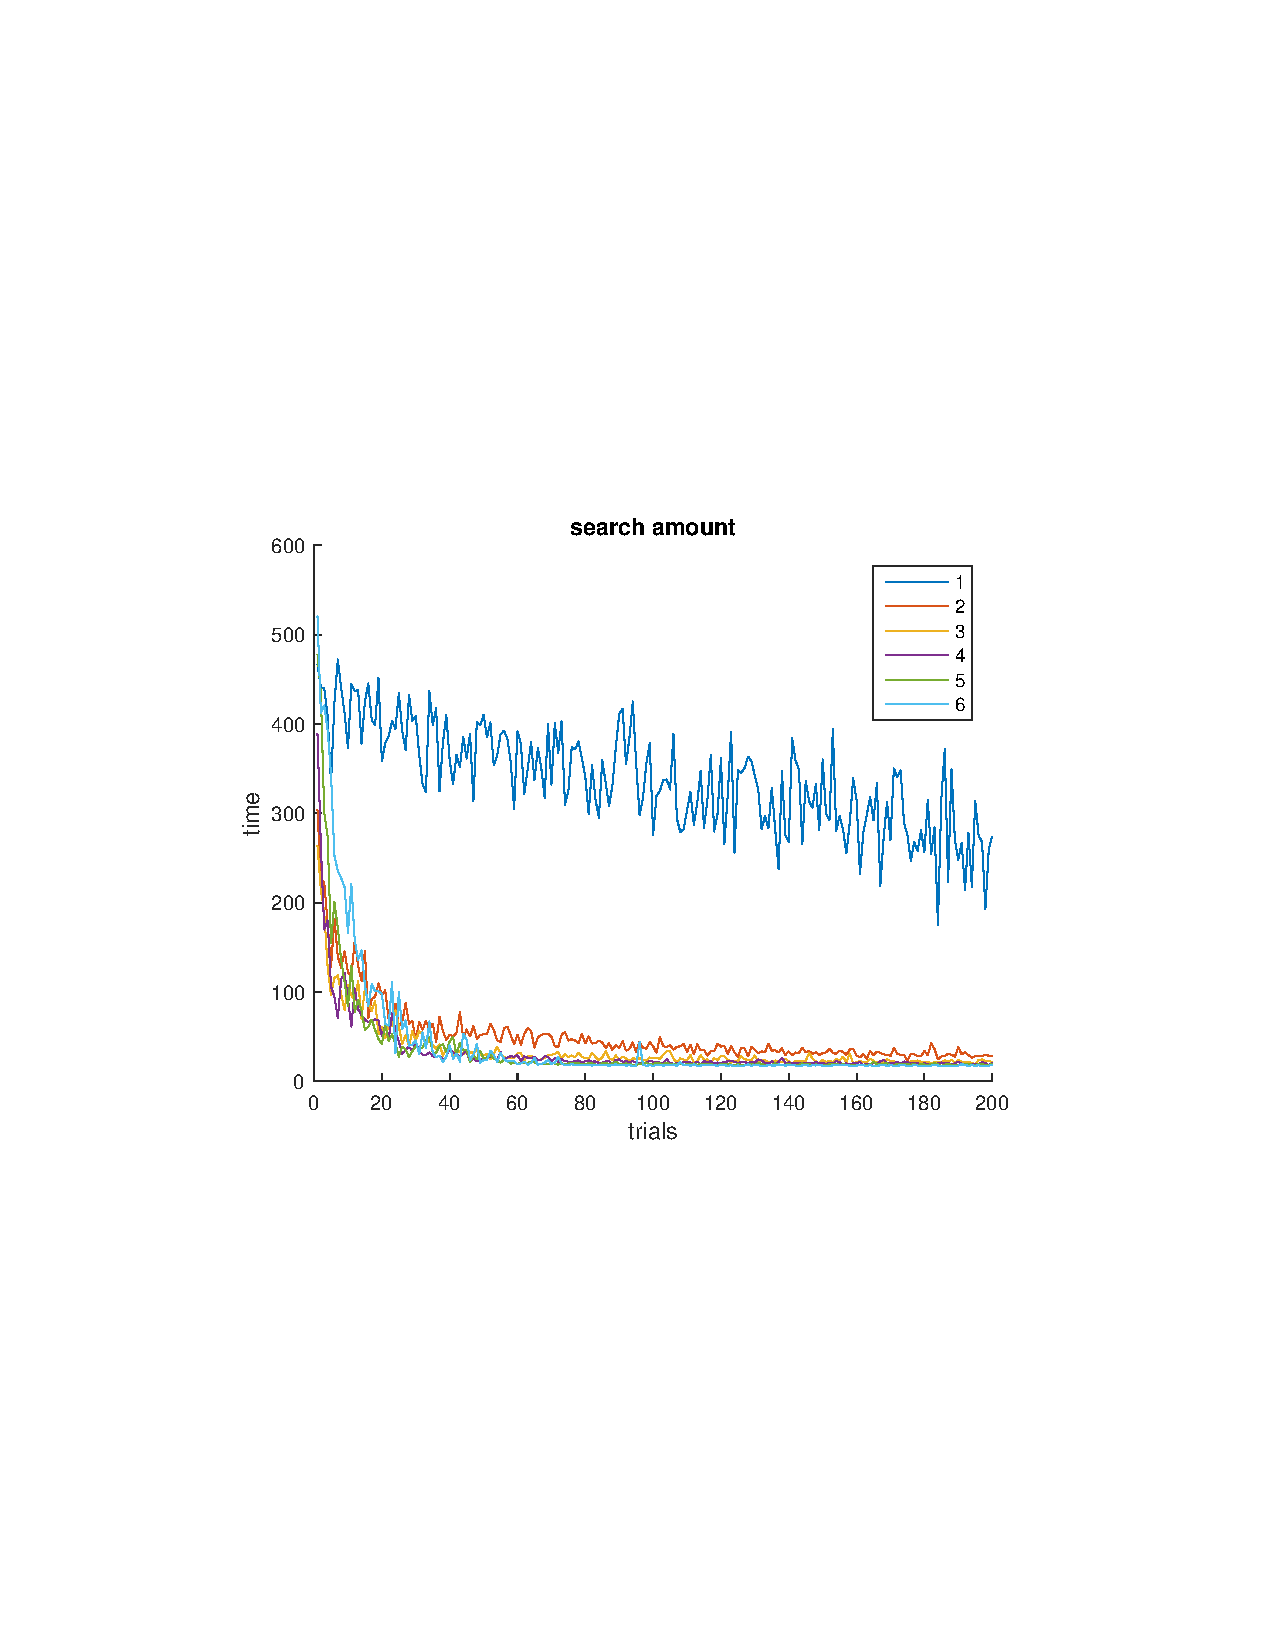
\includegraphics[scale=0.5]{search_changes.pdf}
% \caption{}
% \label{fig:search_changes}
% \end{figure}

\begin{figure*}[h]
    \centering
    \begin{subfigure}[h]{0.49\textwidth}
        \centering
        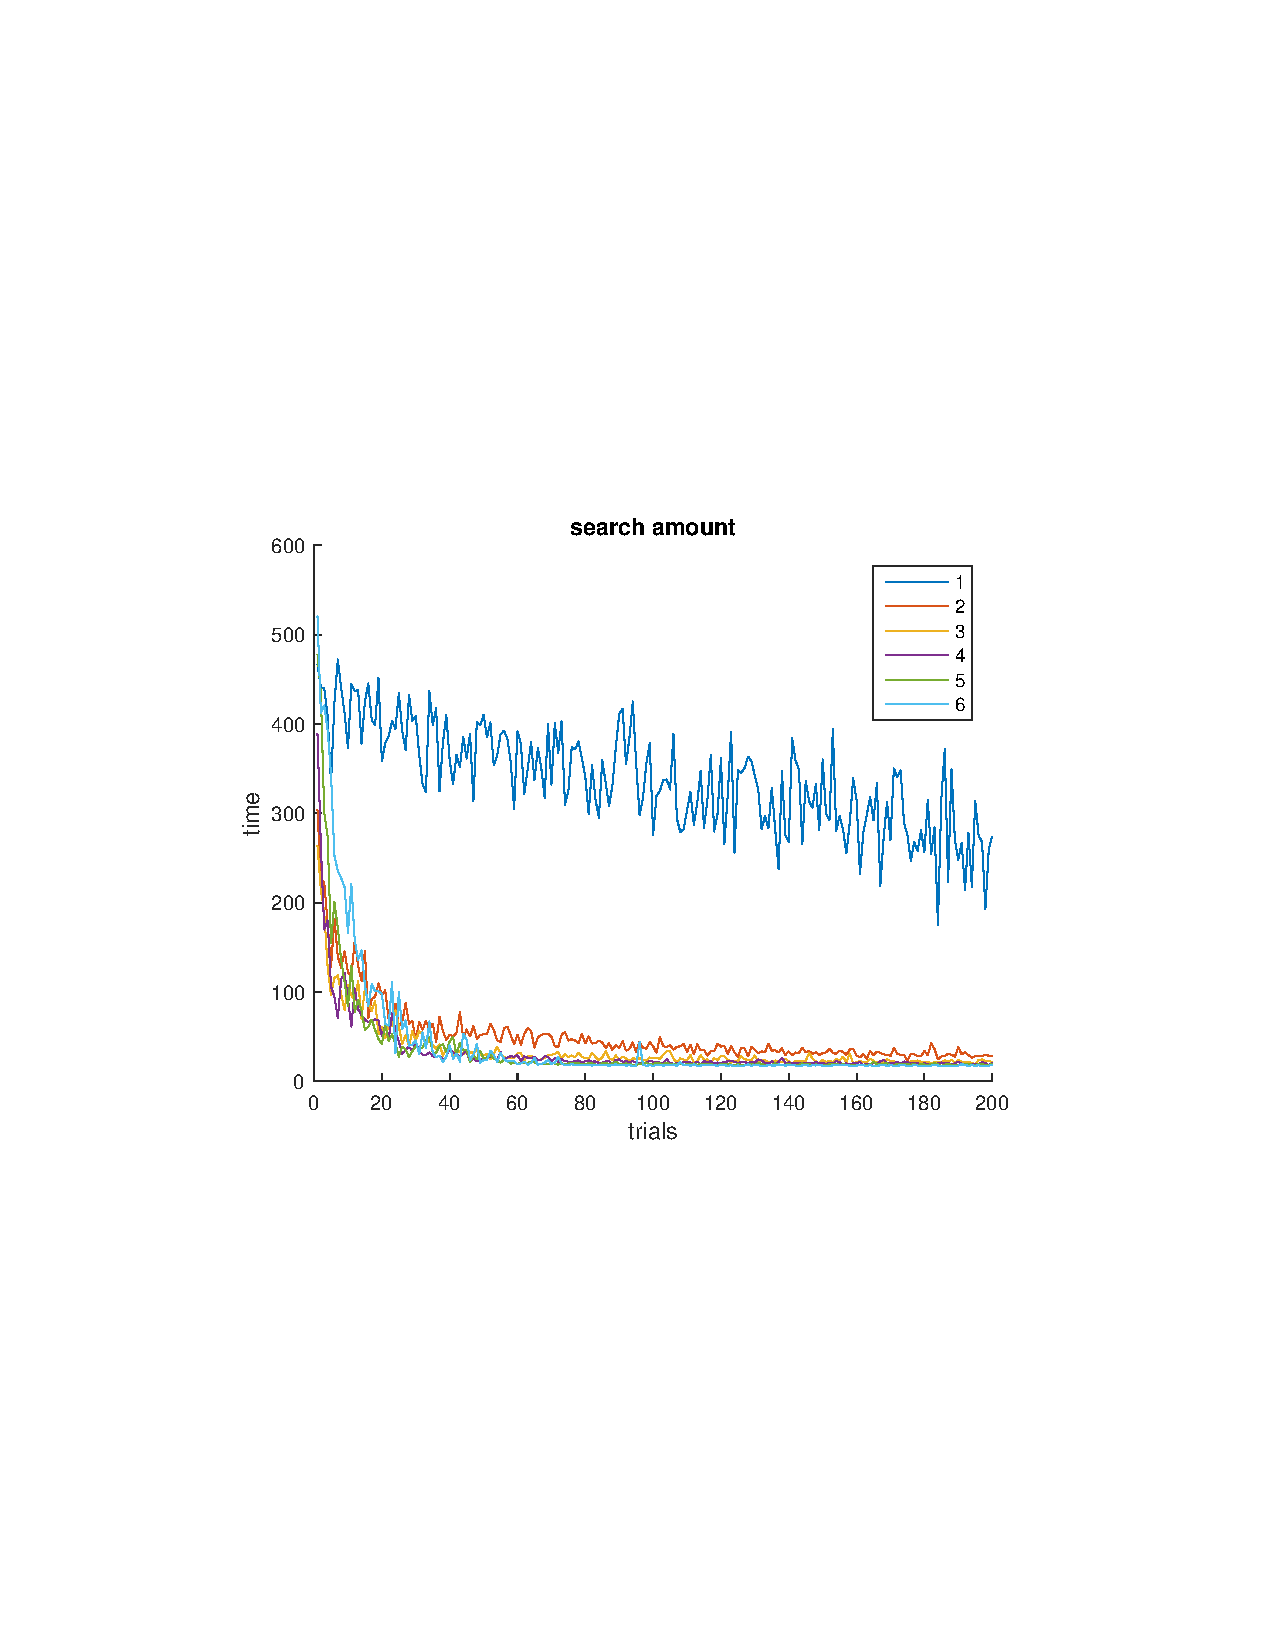
\includegraphics[scale=0.49]{search_changes.pdf}
        \caption{Changes in search attempts per agent move. The line with 1 search attempt denotes the model-free performance. I held the depth constant.}
		\label{fig:search_changes}
    \end{subfigure}%
    ~ 
    \begin{subfigure}[h]{0.49\textwidth}
        \centering
        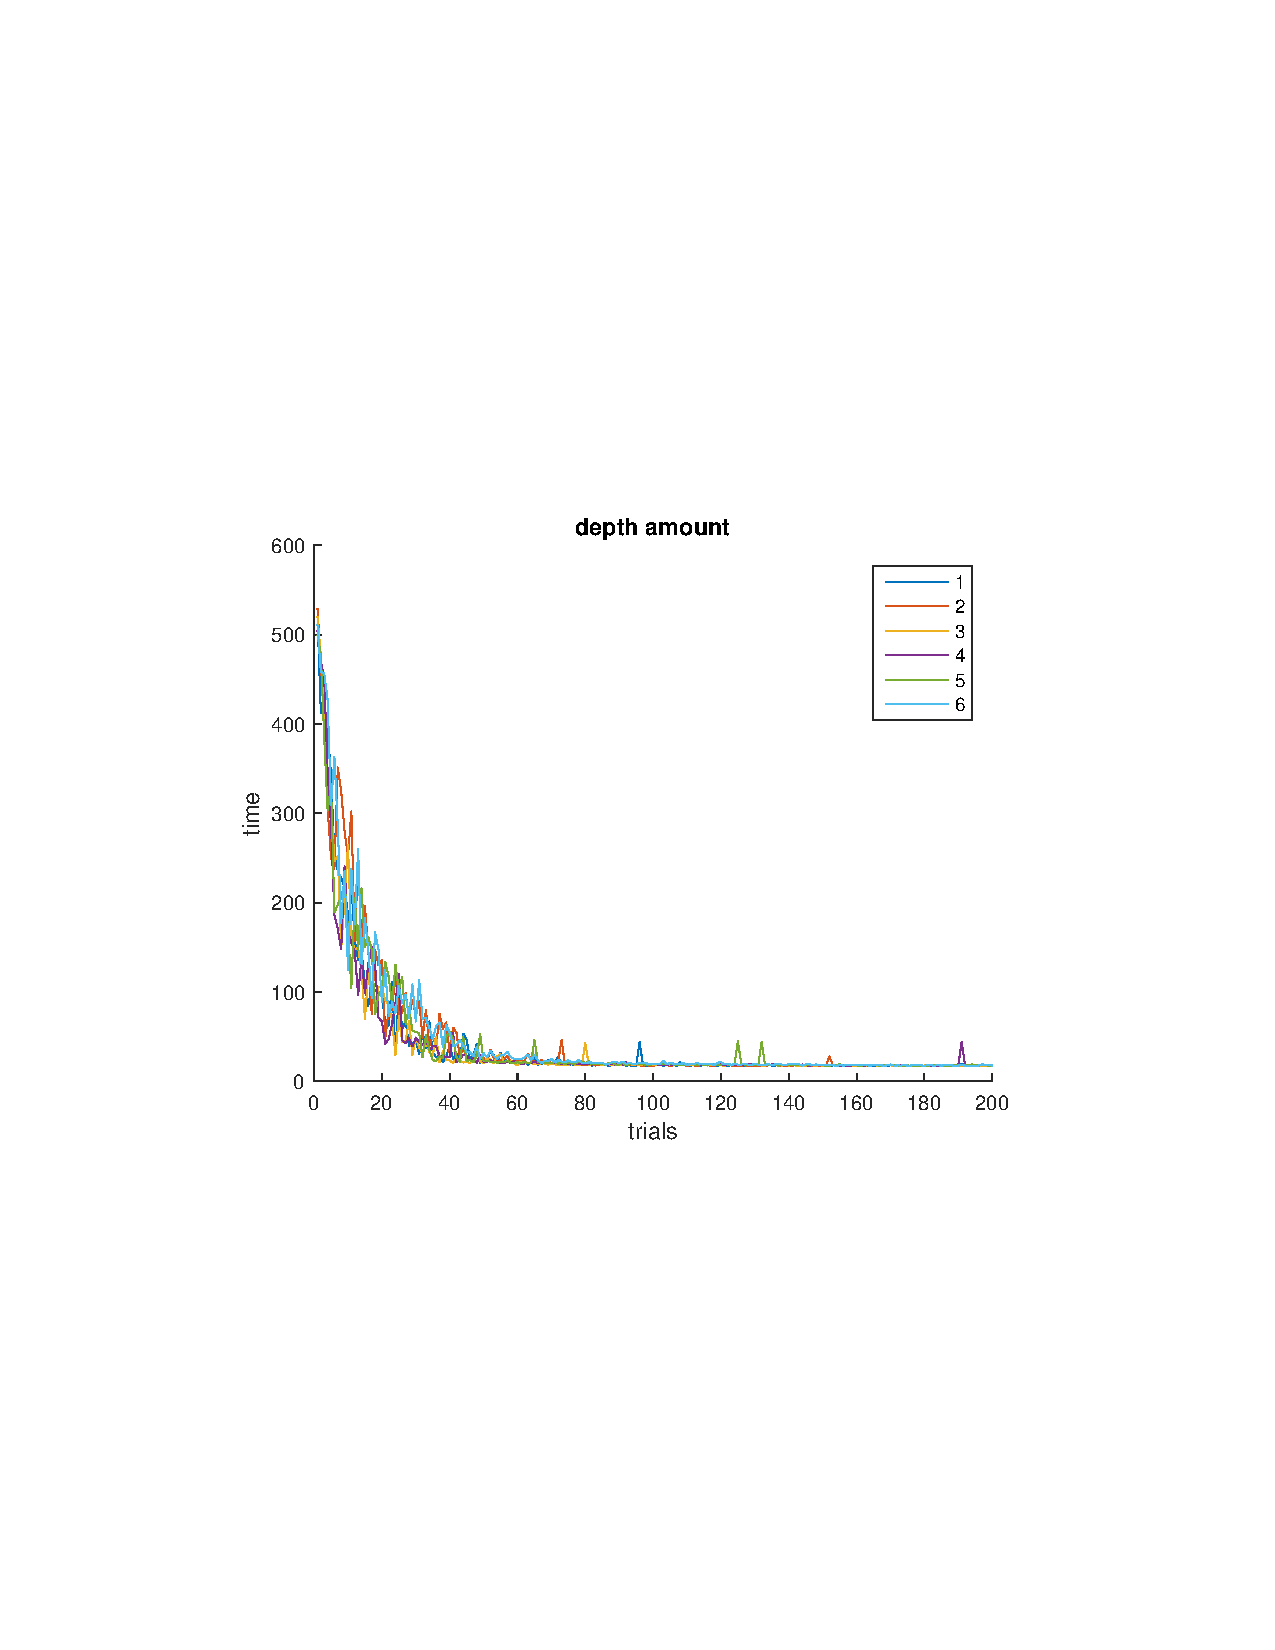
\includegraphics[scale=0.49]{depth_changes.pdf}
        \caption{Depth of the lookahead per agent move. I held the search attempts constant.}
		\label{fig:depth_changes}
    \end{subfigure}
    \caption{Results from my experiments with model based HRL. The first figure shows that that the more search attempts improves the model. I also show that the amount of depth impacting the model is difficult to ascertain.}
\end{figure*}

\section{Discussion}
We performed policy iteration to compare my approach. Policy iteration is a model-free dynamic programming RL technique. Policy iteration finds the optimal path in only a dozen iterations, clearly outperforming my approach. However, in many problems unlike this toy problem I experimented with, the state search space makes dynammic programming approaches intractable, such as with the game GO where the game-tree complexity is approximately $10^{360}$. My approach would perform better in these areas as Alpha Go demonstrated.

Model-based HRL reduces the number of trials for learning the optimal solution in HRL at the cost of additional computational resources and overhead. It is true that HRL will eventually reach the optimal state. However, the cost of computational resources may be outweighed by the cost of performing an action, for example, a robot that must take actions in real time. Thus selecting optimal actions is paramount due to the time lag between execution of actions.

% the reduction in training trials for model-based approaches is beneficial for certain problems. Such as where an where the cost of a trial outweights the cost of computational resources. An example would be a robot that must take actions in real time.
% Explain the reasoning behind the results. Dig into interesting findings here.
% Discuss policy iteration.
% Why not use policy iteration if you know the T and R functions? 
	% I dont use it because my T and R is assumed, but remains unknown. I could easily create a system that predicts the likely next state without actually using a transition function.  it out and say that yes I assume my transition function but what I could do in the future is have the transition predicted or learned itself

\section{Conclusion}
For my future work, we'd like to try different problems to test whether increases in the maximum depth is useful. We'd like to combine deep convolutional networks to approximate both the state of the environment and the transition and reward functions. I would also like to determine ways to automatically generate the options ourselves.